\chapter{Apache Cassandra}
\chapterauthor{David Marchi, Daniel Schäfer, Erik Zeiske}

\section{Introduction}
%- History, relevance, environment, context
%- Task, goal, why, what
%- Structure
\subsection{Abstract}
\subsection{Overview of Cassandra}
Cassandra is a Wide Column Store Database. It is table-like but not relational.
The architecture and design make it a distributed and masterless data store for large data.
It is written in Java and can be run distributed on commodity hardware.
Since it is masterless there is no single point of failure.
Nodes (connected instances running Cassandra) can be hot-swap like conntected to a Cassandra cluster.
This is called elastic scalability. Adding a new node and removing one will elasticly increase or decrease
the cluster size without any major imapct on the distributed system.
All these features make Cassandra highly availabile and fault tolerance.
Depening on the settings, a cluster of Cassandra nodes can be more or less consistent.
From eventually consistent, the lowest setting for consistency, to highly consistent.
This can be reffered to as tunable consistency and allows for a configuration depening classification in 
the CAP Therorem. More on that in another chapter.

Cassandra was originally developed by Facebook in 2008, the co-author of Amazons DynamoDB was involved
in the development process. Cassandra does share similarities to DynamoDB and Googles BigTable approach.
Now it is a free software project of the Apache Foundation. Development is mainly driven by DataStax.
A company designated for commercial Cassandra instances and enterprise support.


\section{Wide Column Store}

A wide column store is a tabular but not relational aproach to store data.
It is not column oriented, since the rows are stored together. 
A row can have missing columns which are not stored on disk. This makes it sparse.
It can be thought like a key-value store where the value can have a subset of a predefined set of columns.
Or put in other words; "Sparse, distributed multi-dimensional sorted map" \cite{chang2008bigtable}
The naming can explained as a key value store with wide (complex) values that consist of columns.


\section{Use-Cases Cassandra}
There are several benefits for using cassandra such as:
\begin{itemize}
        \item Fast writes \\ (high throughput, not latency) \\
        (Those writes include {INSERT} {UPDATE} {DELETE})
        \item High availability
        \item Easy (linear) horizontal scalability
        (The inter-node communication does not increase with more nodes)
        \item No master $\rightarrow$ \\ Read from and write to any node
        \item Flexible schema \\ (rows can have missing columns and missing columns are not stored on disk)
        \item Globally distributed cluster \\ (e.g. multicloud)
        \item Query language similar SQL (CQL)
\end{itemize}
If any of these points apply to a project or use-case Cassandra might be a fit. 
But to be sure it is even more important to rule out the cases where Cassandra is for sure not a fit.
This is the case if:
\begin{itemize}
        \item Single system instance
        \item Ever changing queries (The table is fine-tuned for pre defined queries)
        \item Lots of updates and deletes interspersed with reads (This slows Cassandra down)
        \item Transactions (ACID)
        \item Relations (joins, ...)
        \item Column aggregation ({GROUP BY}) \\
        (Being a wide cloumn oriented database, these functions are not available)
        \item {AUTO INCREMENT}
        \item Data validation (e.g. {NULL} constraint, uniqueness) (It has to be noted, that Cassandra does not read before writing. Any similar needs are not possible)
\end{itemize}

To sump it up there are general Use-Case conditions where Cassandra is a great fit.
Envornments with these needs should find a solution with Cassandra/
\begin{itemize}
    \item Large Deployments
    In order to make use of Cassandras features and benefits 
    \item Tons of writes
      \begin{itemize}
        \item{"high performance at high write volumes with many concurrent client threads" \cite{cassandra_oreilly}}
      \end{itemize}
    \item Geographical distribution of data and database clients
    \item Different columns per row
\end{itemize}
{Ingenuity, architecture and featureset limited when used as single-node}
 {Several nodes? $\rightarrow$ might be a fit}
 {Dozen of nodes? $\rightarrow$ great fit}

{Consider read/write ratio}
    <2>[item]{As mentioned, cassandra optimized for write throughput}
    <2>[item]{Not many updates / data changes, slows read down}
    <2>[item]{Quote; you can even write to multiple nodes with multiple threads}

    <3>[item]{Globally deployed application, bring data to user}
    <3>[item]{Configure to replicate across multiple data centers}

    <4>[item]{Again: rows are sparse}


\section{Data Modelling in Cassandra}  % How to model data (or rather tables)


 
Data Modelling is different in Cassandra, compared to other Databases like traditional 

\section{Using the Cassandra Query Language}  % How to use CQL
This section will give a short overview of how to interact with a Cassandra database using the Cassandra Query Language (CQL), which is mainly inspired by the Structured Query Language (SQL) \autocite{cqlAlexMeng, newInCQL3, cassandra3cqldocCreateKeystore}.

\subsection {Creating a keyspace}
This similarity start by looking into how the creation of a keyspace is performed:
\begin{verbatim}
/* Create a new keyspace in CQL */
CREATE KEYSPACE data WITH replication =
\{'class': 'SimpleStrategy', 'replication_factor': 3\};

/* Create a new database in SQL */
CREATE DATABASE data;
\end{verbatim}
Hereby the only difference is that instead of creating a Database a keyspace is created and it is possible to specify which replication parameters should be used. What these parameter meen and how they should be used is explained later in Section \ref{sec:CassandraClusterArchitecture} \autocite{cqlAlexMeng}.

\subsection{Creating a table}
After creating a keyspace a table has to be created in order to hold the data. As a database is always part of a keyspace it is either necessary to specify the keyspace in every query or to simple scope every subsequent query into a given keyspace by using the USE query \autocite{cassandra3cqldocUse}:
\begin{verbatim}
USE data;
\end{verbatim}

Using this keyspace a table can be created using the same syntax as in SQL \autocite{cqlAlexMeng, newInCQL3, cassandra3cqldocCreateTable}:
\begin{verbatim}
CREATE TABLE groups (
   group_name varchar,
   group_location varchar,
   added_date date,
   username varchar,
   PRIMARY KEY (...)
);
\end{verbatim}

Hereby the only difference is how the primary key can be specified:
\begin{figure}[ht]
    \centering
\begin{verbatim}
      partition key       clustering key  clustering key
       |       |                |            |
((groupname, group_location), added_date, username)
\end{verbatim}
    \caption{Parts of a primary key specification in CQL \autocite{cqlPrimaryKeyDefinition}}
    \label{fig:cassandra:primaryKeyDefinition}
\end{figure}
The first part of the definition will always be the partition key. If it is a compound of several columns they need to be marked by parenthesis separated by comma in order to state that they as a hole build the partition key. If necessary the primary key can be followed by several clustering keys. Keep in mind that the data will be ordered first by the first clustering key after that by the second and so on. This means that a order by has to first called on the first clustering key and the fine ordering can be done on the subsequent one. It will not be possible to only order by the second or other subsequent clustering keys when not ordering by the first \autocite{cqlPrimaryKeyDefinition, cassandra3cqldocCreateTable}.

\subsection{Interacting with data}
In order to manipulate cassandra only provides three possible methods \autocite{cassandra_paper}:
\begin{itemize}
    \item insert(table, key, rowMutation)
    \item get(table, key, columnName)
    \item delete(table, key, columnName)
\end{itemize}
All having in common that the whole primary key has to be specified in order to interact with the data. The only exception hereby is the getting of data where only the partition key has to be specified.

Important to note is that there is no interaction to update a data entry. The reason for that is that as Cassandra is optimized for high write throughput is is very costly to read any data before writing. This means that an update and insert known from SQL will perform the same action on the data \autocite{cqlAlexMeng, newInCQL3}:
\begin{verbatim}
/* Inserting Data */
INSERT INTO Person (lastname, name, email)
VALUES ('Musterfrau', 'Maxi', 'maxi@gmail.com');

/* Updating Data */
UPDATE Person SET email = 'maxi@gmail.com'
WHERE lastname='Musterfrau' AND name = 'MAXI';
\end{verbatim}

As getting and deleting data is also similar to SQL there is no need to go into it any further in this section \autocite{cqlAlexMeng, cassandra3cqldocSelect}:
\begin{verbatim}
/* Selecting Data */
SELECT * FROM Person
  WHERE lastname='Musterfrau' AND name = 'Maxi';
/* Deleting Data */
DELETE FROM Person
  WHERE lastname='Musterfrau' AND name = 'Maxi';
\end{verbatim}

\section{Local reads and writes}
In order to perform the requested changed to the data they have to be written into the database. This section will take a look into how the changes will be written on a single node not taken into account the cluster.

\begin{figure}[ht]
    \centering
    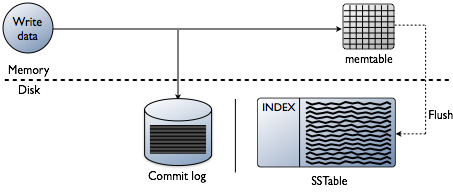
\includegraphics[width=0.75\textwidth]{img/cassandra_local_write.png}
    \caption{Writing data to Cassandra node \autocite{datastaxWriteData}}
    \label{fig:cassandra:writeData}
\end{figure}
In figure \ref{fig:cassandra:writeData} it can be seen that the write processe to cassadra involves three steps:
\begin{enumerate}
\item \textbf{Write to journal} Hereby the query is simple append to the journal on the disk, making it persistent even if the node goes down. As this action is a simple append it is very fast and leaves the data in a temporal order in the journal.
\item \textbf{Write to memtable} After writing to the journal the change is performed in the memtable putting the data into a Sorted String Table (SSTable). This form is the same form the data will be written on disk,
\item \textbf{Flush to disk when memtable is too big} This allows to simple flush the data and some metadata to the disk when it gets to big for the memory to hold it. Hereby a new data file is created not touching any of the previously written files, making this action also quite fast as no lookups have to be performed.
\end{enumerate}

After writing the data it also can be read again as shown by figure \ref{fig:cassandra:readData}:
\begin{figure}[ht]
    \centering
    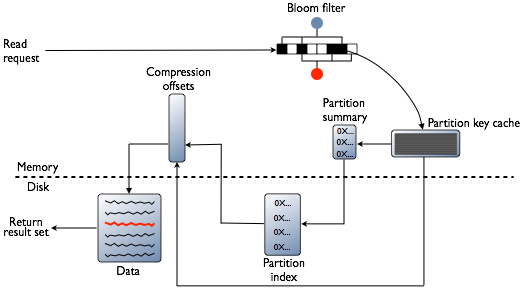
\includegraphics[width=0.75\textwidth]{img/cassandra_local_read.png}
    \caption{Reading data from Cassandra node \autocite{datastaxReadData}}
    \label{fig:cassandra:readData}
\end{figure}
\begin{enumerate}
    \item \textbf{Check caches} First the last query cache will be checked. Returning the data right away if it was requested in the near past.
    \item \textbf{Check memtable} Afterwards the memtable will be checked if it has recent activities on the requested data.
    \item \textbf{Find SSTable and location} If no entry was found in the memtable the data on disk will be checked by firstly determining in which memtable dump the dataset will be and then retriving it from there.
    \item \textbf{Merge with memtable} If it was necessary to retrieve the data from disk the data will be written to the memtable to allow later queries on the same data to succeed erlier.
\end{enumerate}

\section{Cluster Architecture}\label{sec:CassandraClusterArchitecture}  % How the cluster works
This is the cluster architecture

\newcommand{\Ray}{3cm}
\begin{figure}[ht]
  \begin{tikzpicture}
    % Nodes on the circles
    \node[circle,minimum width=2cm,minimum height=1cm,draw,name path=n1] (Node A) at (90:\Ray) {A};
    \node[circle,minimum width=2cm,minimum height=1cm,draw,name path=n2] (Node B) at (0:\Ray) {B};
    \node[circle,minimum width=2cm,minimum height=1cm,draw,name path=n3] (Node C) at (270:\Ray) {C};
    \node[circle,minimum width=2cm,minimum height=1cm,draw,name path=n4] (Node C) at (180:\Ray) {D};

    % Circle the nodes are placed on
    \path[name path=c] circle (\Ray);
    \path[name intersections={of=n1 and c,name=i1},
          name intersections={of=n2 and c,name=i2},
          name intersections={of=n3 and c,name=i3},
          name intersections={of=n4 and c,name=i4}
         ];

    % Arrows between the nodes
    \begin{scope}
      \pgfsetarrowsend{Stealth[scale=1.5]}

      \pgfpathmoveto{\pgfpointanchor{i1-2}{center}}
      \pgfpatharcto{\Ray}{\Ray}{0}{0}{0}{\pgfpointanchor{i2-1}{center}}
      \pgfusepath{draw}

      \pgfpathmoveto{\pgfpointanchor{i2-2}{center}}
      \pgfpatharcto{\Ray}{\Ray}{0}{0}{0}{\pgfpointanchor{i3-1}{center}}
      \pgfusepath{draw}

      \pgfpathmoveto{\pgfpointanchor{i3-2}{center}}
      \pgfpatharcto{\Ray}{\Ray}{0}{0}{0}{\pgfpointanchor{i4-2}{center}}
      \pgfusepath{draw}

      \pgfpathmoveto{\pgfpointanchor{i4-1}{center}}
      \pgfpatharcto{\Ray}{\Ray}{0}{0}{0}{\pgfpointanchor{i1-1}{center}}
      \pgfusepath{draw}
    \end{scope}

    % Labels on arrows
    \node[fill=white] at (45:\Ray) {0 to 63};
    \node[fill=white] at (135:\Ray) {64 to 127};
    \node[fill=white] at (225:\Ray) {128 to 191};
    \node[fill=white] at (315:\Ray) {192 to 255};
  \end{tikzpicture}
  \caption{Token Ring}
  \label{fig:cassandra:tokenring}
\end{figure}

\section{Distributed writes and reads (CAP Theorem)}

\section{Setup and Configuration}  % Setup

\section{Summary and Conclusion}
